\documentclass{article}
\usepackage[utf8]{inputenc}
\usepackage[a4paper, total={6in, 8in}]{geometry}
\usepackage{graphicx}
\usepackage{amsmath}
\usepackage{enumitem}

\title{Econ 20000-Problem Set 6}
\author{Dr. Fulya Ersoy}
\date{}
\begin{document}
\maketitle
\begin{enumerate}
\item (based on exercise 10.11 from Lima) Patrick owns a candy shop. He sells hard and soft candies, but also consumes them. Patrick orders his preferences for hard and soft candies according to the following utility function:
$$U(h, s) = 150h - h^2 + 300s - 2s^2$$
Assume that Patrick's customers can purchase any quantity of hard and soft candies.
 \begin{enumerate}[label=(\alph*)]
 \item  Suppose that Patrick is given the opportunity to consume as many pounds of hard candy and as many pounds of soft candy as he desires, regardless of cost. How much candy does Patrick consume?
 \item[] $\frac{\partial U}{\partial h}=150-2h=0\Rightarrow h^*=75$, $\frac{\partial U}{\partial s}=300-4s=0\Rightarrow s^*=75$, therefore $(h,s)=(75,75)$.
 \item Suppose that the price of a pound of hard candy is 4 dollars and the price of a pound of soft candy is 2 dollars. Patrick's bakery produces 60 pounds of hard candy and 100 pounds of soft candy every day. Draw the budget constraint in red ink and label the initial endowment point E.
 \item[] $E=(60,100),\; p_h=4, \; p_s=2\Rightarrow 4h+2s=4\cdot60+2\cdot100=240+200=440$.
 \item[] When $s=0\Rightarrow 4h=440\Rightarrow h=110$. When $h=0\Rightarrow 2s=440\Rightarrow s=220$.
 \item[] Constraint drawn:
 \item[] 
 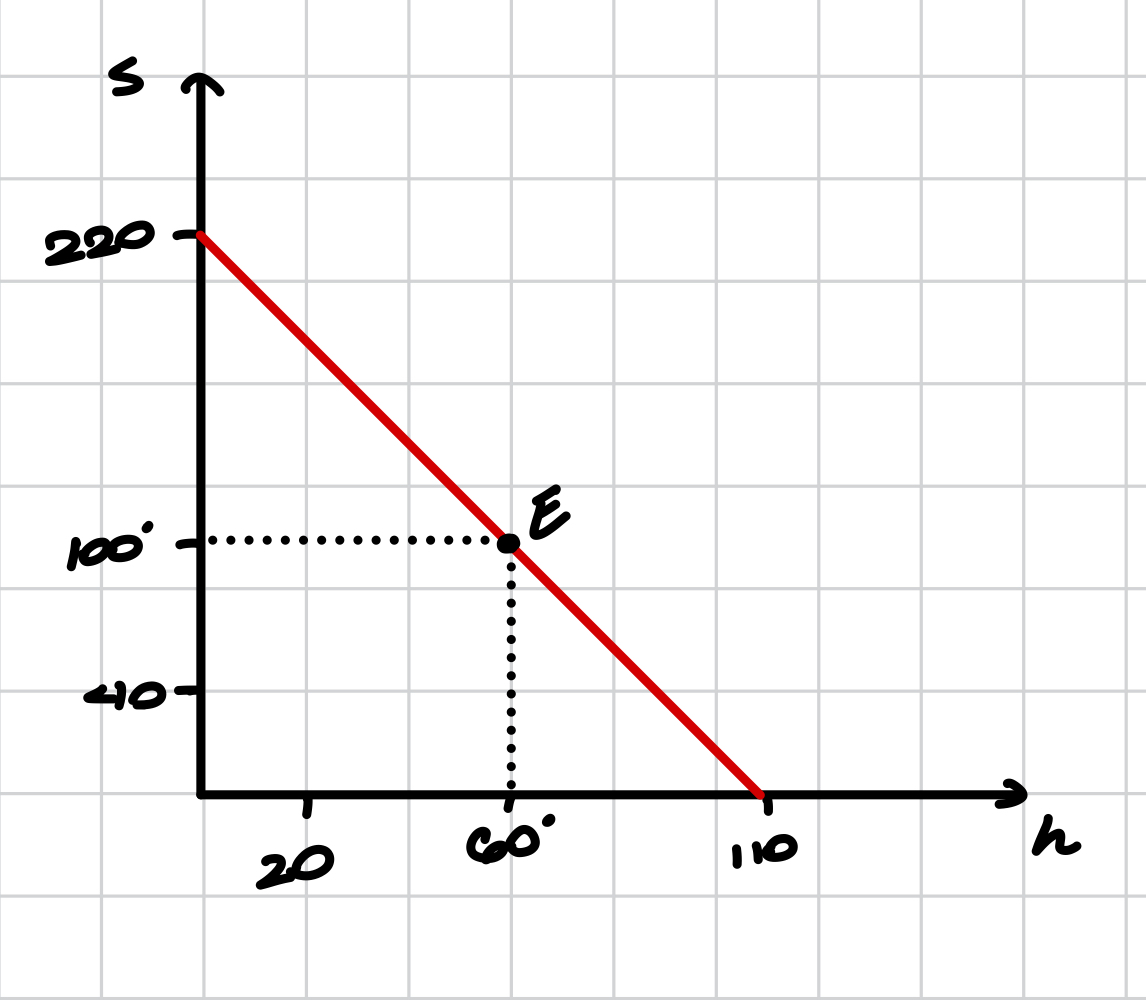
\includegraphics[width=7cm]{ECON 20000 PSet 6 Image 1.jpeg}
 \item Is the answer you found in part (a) feasible with these prices?
 \item[] $h=75,\;s=75\Rightarrow 4\cdot75+2\cdot75=450>440$. Therefore, answer in part (a) not feasible.
 \item Solve Patrick's utility maximization problem. Find the optimal consumption bundle O. Is Patrick net buyer or net seller of hard candy? Is Patrick net buyer or net seller of soft candy?
 \item[] $\max_{h,s}U(h,s)=150h-h^2+300s-2s^2$ s.t. $4h+2s=440$.
 \item[] $\mathcal{L}=150h-h^2+300s-2s^2+\lambda(440-4h-2s)$.
 \item[] FOC's: $\begin{cases}
     \frac{\partial\mathcal{L}}{\partial h} = 150-2h-4\lambda=0 \\ \frac{\partial\mathcal{L}}{\partial s} = 300-4s-2\lambda=0\\ \frac{\partial\mathcal{L}}{\partial\lambda} = 440-4h-2s=0
 \end{cases}$. 
 \item[] From first two conditions: $2h=150-4\lambda\Rightarrow h=75-2\lambda$, $4s=300-2\lambda\Rightarrow s=75-\frac{\lambda}{2}$.
 \item[] Solve $\lambda$: $4(75-2\lambda)+2(75-\frac{\lambda}{2})=440\Rightarrow 300-8\lambda+150-\lambda=440\Rightarrow 9\lambda=10\Rightarrow\lambda = \frac{10}{9}$.
 \item[] Then, $h^*=75-2(\frac{10}{9})=72.78$, $s^*=75-\frac{1}{2}\cdot\frac{10}{9}=74.44$, O$^*$ $=(h^*,s^*)=(72.78,74.44)$.
 \item[] $72.78>60$, and $74.44<100$. Thus, Patrick is a net buyer of $h$, and a net seller of $s$.
 \item Suppose that the price of a pound of hard candy falls to 2 dollars before Patrick sells his endowment. Draw the new budget line in blue ink. Does Patrick's demand for hard candy rise or fall? By how much? What happens to his demand for soft candy?
 \item[] $E=(60,100), \; p_h=2, \; p_s=2\Rightarrow2\cdot60+2\cdot100=320$.
 \item[] When $s=0\Rightarrow2h=320\Rightarrow h=160$. When $h=0\Rightarrow 2s=320\Rightarrow s=160$.
 \item[] Constraint drawn:
 \item[]
 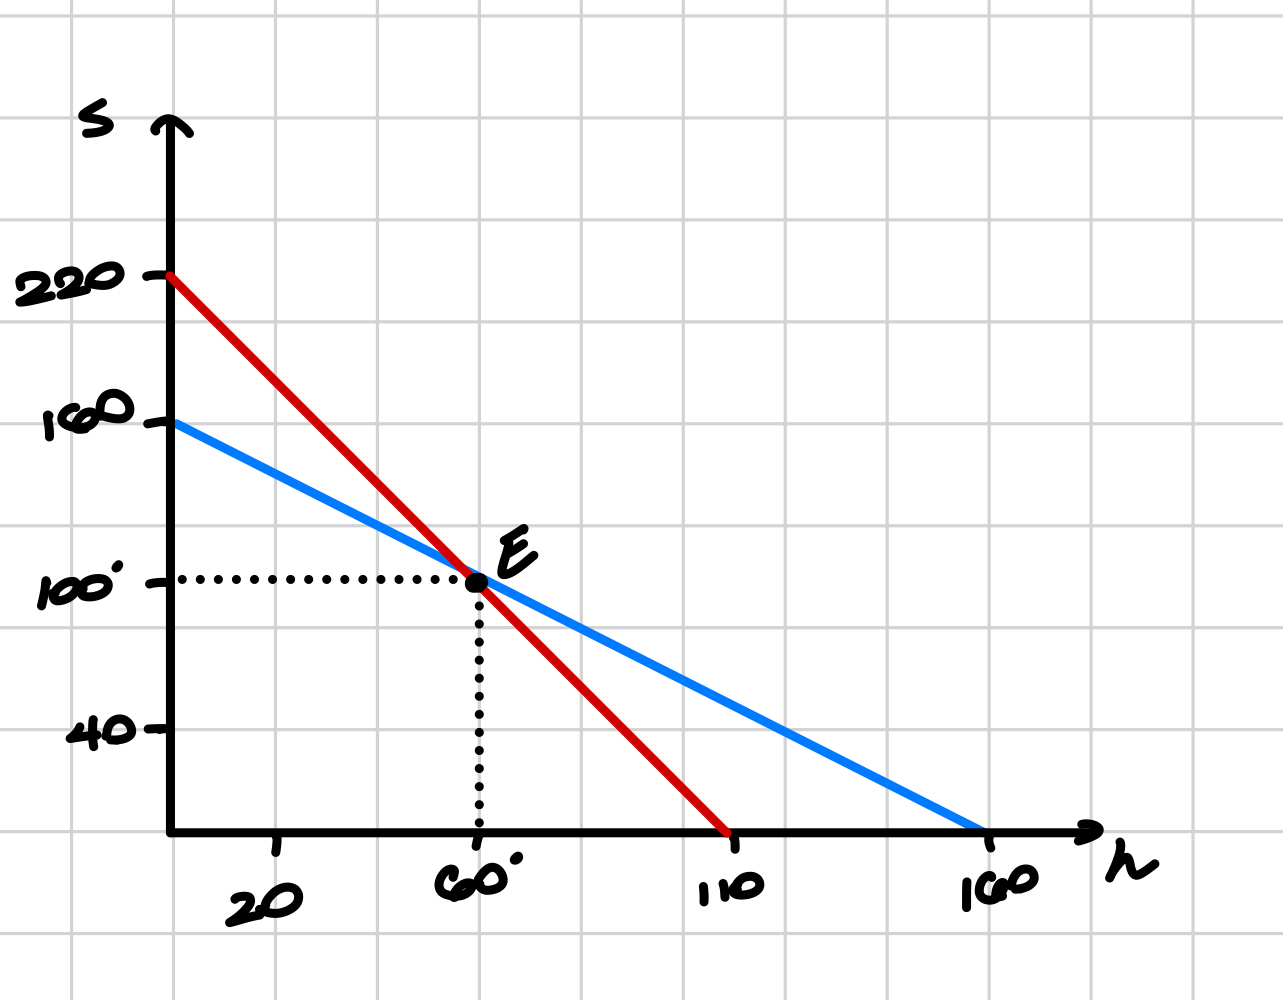
\includegraphics[width=7cm]{ECON 20000 PSet 6 Image 2.jpeg}
 \item[] $\max_{h,s}U(h,s)=150-h^2+300s-2s^2$ s.t. $2h+2s=320$
 \item[] $\mathcal{L}=150-h^2+300s-2s^2+\lambda(320-2h-2s)$
 \item[] FOC's: $\begin{cases}
     \frac{\partial\mathcal{L}}{\partial h} = 150-2h-2\lambda=0 \\ \frac{\partial\mathcal{L}}{\partial s} = 300-4s-2\lambda=0\\ \frac{\partial\mathcal{L}}{\partial\lambda} = 320-2h-2s=0
 \end{cases}$. 
 \item[] From first two conditions: $2h=150-2\lambda\Rightarrow h=75-\lambda$, $4s=300-2\lambda\Rightarrow s=75-\frac{\lambda}{2}$.
 \item[] Solve $\lambda$: $2(75-\lambda)+2(75-\frac{\lambda}{2})=320\Rightarrow150-2\lambda+150-\lambda=320\Rightarrow 3\lambda=-20\Rightarrow\lambda=-\frac{20}{3}$.
 \item[] Then, $h'=75-(-\frac{20}{3})=81.67$, $s'=75-(\frac{1}{2})\cdot(-\frac{20}{3})=78.33$, O' $=(h',s')=(81.67,78.33)$.
 \item[] $\Delta h=h'-h^*=81.67-72.78=8.89$. Thus demand for $h$ increases by 8.89 pounds.
 \item[] $\Delta s=s'-s^*=78.33-74.44=3.89$. Thus demand for $s$ increases by 3.89 pounds.
 \item Is Patrick better off or worse off after price change? How do you know?
 \item[] $U$(O$^*$)$=150(72.78)-(72.78)^2+300(74.44)-2(74.44)^2=16871.235$.
 \item[] $U$(O')$=150(81.67)-(81.67)^2+300(78.33)-2(78.33)^2=16807.500$.
 \item[] Since $U$(O')\;$<$\;$U$(O$^*$), Patrick is worse off after price change.
\item What is the endowment effect of price change on hard candy?
\item[] Endowment effect: $h^f-h^I$ where $h^I=h_m(p_h^f,p_s,m=m^0)$ and $h^f=h'$.
\item[] $\Rightarrow 2(75-\lambda)+2(75-\frac{\lambda}{2})=440\Rightarrow 150-2\lambda+150-\lambda=440\Rightarrow 3\lambda=-140\Rightarrow\lambda=-\frac{140}{3}$.
\item[] $\Rightarrow h^I=75-\frac{-140}{3}=121.67$, $h^f=h'=81.67$. Endowment effect $=81.67-121.67=-40$.
\end{enumerate}
\end{enumerate}
\begin{enumerate}
   \setcounter{enumi}{1}
\item  Edgeworth Box: Consider a 2-consumer, 2-good pure exchange economy. Suppose that Consumer A has endowment $\omega_A = (4,2)$ and Consumer B has endowment $\omega_B = (2,3)$. Suppose further that Consumer A has preferences represented by the utility function $U_A (x, y ) =x y$ and Consumer B has preferences represented by the utility function $U_B (x, y ) = x + y$.
\begin{enumerate}[label=(\alph*)]
\item Draw the Edgeworth Box for this economy. Label the endowment point and draw the indifference curve that passes through the endowment point for each consumer.
\item[] 
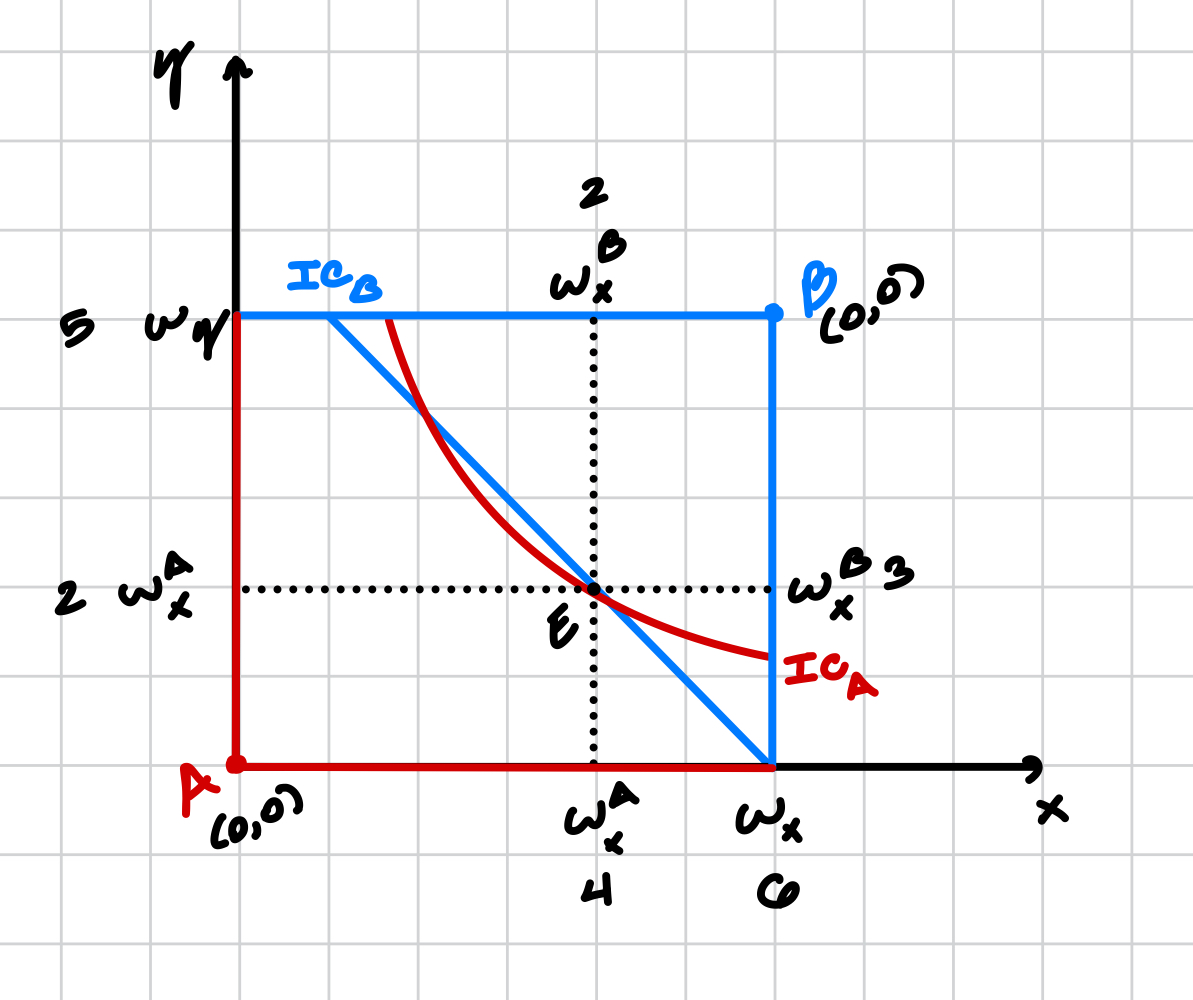
\includegraphics[width=7cm]{ECON 20000 PSet 6 Image 3.jpeg}
\item Find (analytically) the Contract Curve. Draw it in the Edgeworth box.
\item[] For A: $MRS_A=\frac{MU_x}{MU_y}=\frac{y}{x}$. For B: $MRS_B=\frac{MU_x}{MU_y}=\frac{1}{1}=1$. $MRS_A=MRS_B$:
\item[] $\Rightarrow\frac{y}{x}=1\Rightarrow y=x$. Thus Contract Curve(CC) $=\{(x_A,y_A):y_A=x_A, \; 0\leq x_A\leq 5\}$.
\item[]
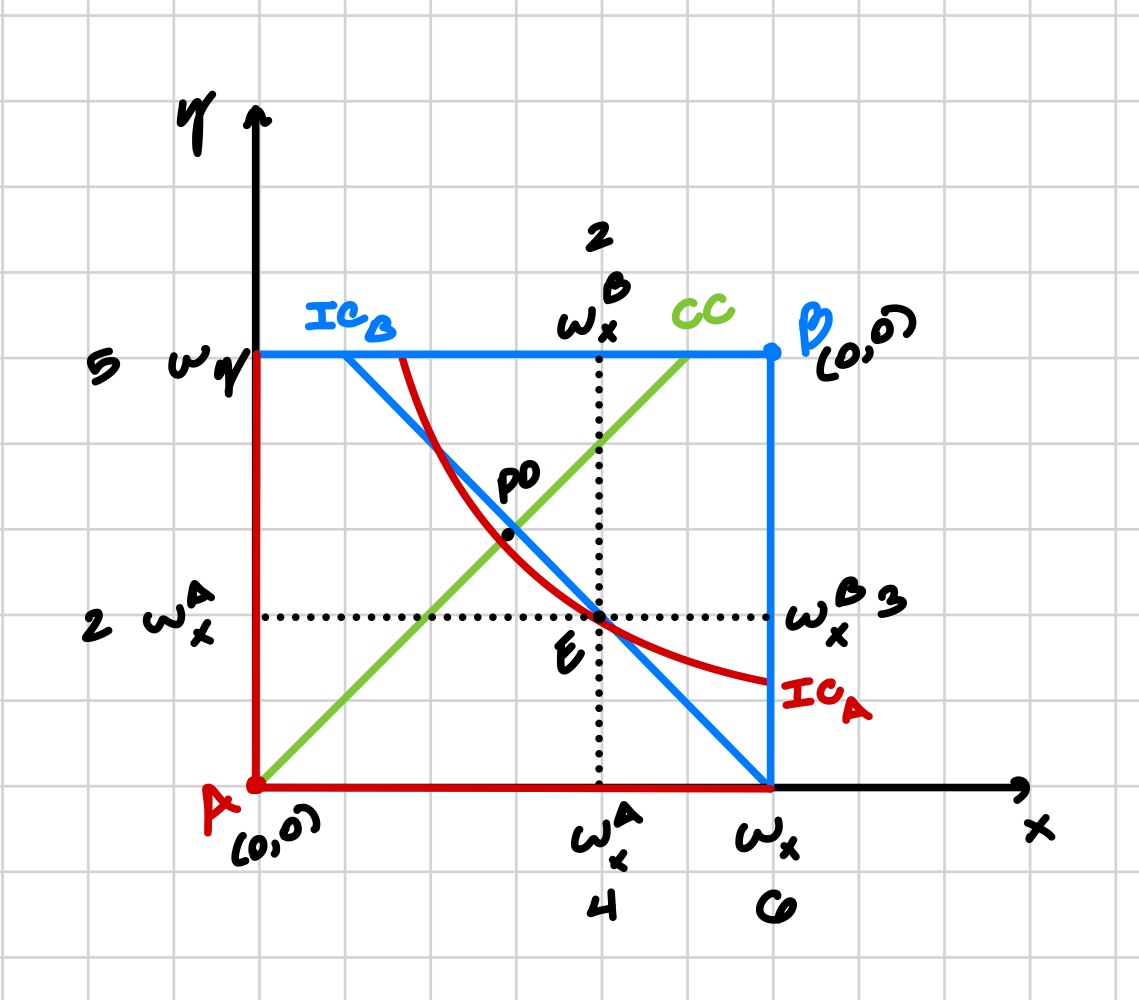
\includegraphics[width=7cm]{ECON 20000 PSet 6 Image 4.jpeg}
\item Find the competitive equilibrium prices (ratio) and allocation.
\item[] Indicated shown as PO, equilibrium allocation is $(x_A,y_A)=(3,3)$ and $(x_B,y_B)=(3,2)$.
\item[] For price ratio: Let $p=\frac{p_x}{p_y}$. Normalize $p_y=1$ so $p=p_x$. For consumer A, utility $xy$ is log-homothetic and Cobb-Douglas with equal shares implies A spends half of wealth on each good. $W_A=p\cdot 4+1\cdot 2=4p+2$. Then, $x_A=\frac{1}{2}\frac{W_A}{p}=\frac{1}{2}(\frac{4p+2}{p})=2+\frac{1}{p}$, and $y_A=\frac{1}{2}W_A=\frac{1}{2}(4p+2)=2p+1$. For consumer B, linear utility $x+y$ gives $MRS_B=1$, so B will buy only the cheaper good or will be indifferent if $p=1$. Suppose $p=1$, then $W_A=4\cdot 1+2=6$, $x_A=2+1=3$, $y_A=2+1=3$, thus $(x_A,y_A)$ is indeed $(3,3)$. Total endowment is $X=6$, $Y=5$, so $x_B=6-x_A=3$, and $y_B=5-y_B=2$, thus $(x_B,y_B)$ is indeed $(3,2)$. Further, $x_B+y_B=5=W_B$ where $W_B=1\cdot 2+1\cdot 3=5$. Hence, B is indifferent and can choose $(3,2)$. Here, markets clear and  equilibrium price ratio is $1:1$.
\end{enumerate}
\item (Based on exercise 28.3 of Lima) Consider a two good, two individual endowment economy. Suppose that individual i's endowment is given by: $\omega^i=(\omega_x^i, \omega_y^i)$ and individual j's, endowment is given by: $\omega^j=(\omega_x^j, \omega_y^j)$. where we assume that $\omega_x^i>\omega_x^j$ and $\omega_y^j>\omega_y^i$. Also assume individual i's preferences are given by: $U (x_i, y_i) = \alpha ln (x_i) + (1 - \alpha) ln (y_i)$ and individual j's preferences are given by: $U (x_j, y_j) = \gamma ln (x_j) + (1 - \gamma) ln (y_j)$. Finally, let the absolute prices of good x and good y be given by $p_x$ and $p_y$.
\begin{enumerate}[label=(\alph*)]
\item Write down each individual's maximization problem.
\item[] Ind i: $\max_{w_x^i,w_y^i}U(x_i,y_i)=\alpha ln(x_i)+(1-\alpha)ln(y_i)$ s.t. $p_xx_i+p_yy_i=p_xw_x^i+p_yw_y^i\equiv W_i$.
\item[] Ind j: $\max_{w_x^j,w_y^j}U(x_j,y_j)=\gamma ln(x_j)+(1-\gamma)ln(y_j)$ s.t. $p_xx_j+p_yy_j=p_xw_x^j+p_yw_y^j\equiv W_j$.
\item Solve each individual's maximization problem. You should obtain $x_i^*$, $x_j^*$, $y_i^*$ and $y_j^*$
\item[] Per Cobb-Douglas spending shares: $x^*_i=\frac{\alpha W_i}{p_x}$, $y^*_i=\frac{(1-\alpha)W_i}{p_y}$, $x^*_j=\frac{\gamma W_j}{p_x}$, $y^*_j=\frac{(1-\gamma)W_j}{p_y}$.
\item Find $x^*$ and $y^*$, aggregate demands for the two goods.
\item[] $x^*=x^*_i+x^*_j=\frac{\alpha W_i}{p_x}+\frac{\gamma W_j}{p_x}=\alpha(w_x^i+\frac{1}{p}w_y^i)+\gamma(w_x^j+\frac{1}{p}w_y^j)$.
\item[] $y^*=y^*_i+y^*_j=\frac{\alpha W_i}{p_y}+\frac{\gamma W_j}{p_y}=(1-\alpha)(pw_x^i+w_y^i)+(1-\gamma)(pw_x^j+w_y^j)$.
\item What are the equilibrium conditions for this economy?
\item[] Equilibrium conditions: $\begin{cases}
    x^*=w_x^i+w_x^j \\ y^*=w_y^i+w_y^j
\end{cases}$
\item Use the the market clearing condition in the x - market to find the equilibrium price. Hint: You can't find absolute prices separately. You need to find the relative price, $p=\frac{p_x}{p_y}$.
\item[] $x^*=\alpha(w_x^i+\frac{1}{p}w_y^i)+\gamma(w_x^j+\frac{1}{p}w_y^j)=\alpha w_x^i+\gamma w_x^j+\frac{1}{p}(\alpha w_y^i+\gamma w_y^j)=w_x^i+w_x^j$
\item[] $\Rightarrow\frac{1}{p}(\alpha w_y^i+\gamma w_y^j)=(w_x^i-\alpha w_x^i)+(w_x^j-\gamma w_x^j)\Rightarrow p^*=\frac{\alpha w_y^i+\gamma w_y^j}{(w_x^i-\alpha w_x^i)+(w_x^j-\gamma w_x^j)}=\frac{\alpha w_y^i+\gamma w_y^j}{(1-\alpha)w_x^i+(1-\gamma)w_x^j}$.
\item Use the market clearing condition in the y - market to find the equilibrium price. You should find that your answer is the same as in part (e). 
\item[] $y^*=p((1-\alpha)w_x^i+(1-\gamma)w_x^j)+(1-\alpha)w_y^i+(1-\gamma)w_y^j=w_y^i+w_y^j$
\item[] $\Rightarrow p((1-\alpha)w_x^i+(1-\gamma)w_x^j)=w_y^i+w_y^j-(1-\alpha)w_y^i-(1-\gamma)w_y^j\Rightarrow p^*=\frac{\alpha w_y^i+\gamma w_y^j}{(1-\alpha)w_x^i+(1-\gamma)w_x^j}$.

\end{enumerate}
\end{enumerate}
\end{document}



a. Define the competitive equilibrium of the endowment economy.
b. Write down each individual's maximization problem.
c. Solve each individual's maximization problem. You should obtain af, yf, and ni for
i = 1,2 where ni denotes the Lagrange multiplier on individual is budget constraint.
d. Find X* and Y", the aggregate demands for the two goods.
e. What are the equilibrium conditions for this economy?
f. Find the market clearing relative price for the r - market.
g. Now use the market clearing condition in the y - market to find the equilibrium price.
How much of good y does each individual consume?